\section{Introduction}
\label{sec:introduction}
% Consider two programs that implement the type isomorphism {$A + (B + C) \isoone C + (B + A)$}, written as two different
% sequences of primitive isomorphisms:

Consider two programs that implement the same type isomorphim:
\begin{align*}
      A + (B + C) \isoone
      (A + B) + C & \isoone
      C + (A + B) \isoone
      C + (B + A)
      \\
      A + (B + C) \isoone
      A + (C + B) \isoone
      (A + C) + B & \isoone
      (C + A) + B \isoone
      C + (A + B) \isoone
      C + (B + A)
\end{align*}

These permutations are written as sequences of primitive operations: associativity, symmetry, and composition. Can we
find necessary and sufficient equations to identify \emph{all} such equivalent sequences of type isomorphisms?

Reversible boolean circuits, which are at the core of quantum computing, are typically formalised as permutations
$\{0,1\}^k \to \{0,1\}^k$ on bit strings of some length $k$~\cite{aaronson_et_al:LIPIcs:2017:8173,1201583}. From the
perspective of programming languages, reversible circuits can be more conveniently expressed as isomorphisms over
algebraic datatypes. The $\PiLang$ family of languages were developed by~\citet*{James:2012:IE:2103656.2103667,theseus}
for writing reversible programs, whose syntax is inspired by the sound and complete axiomatisation of type
isomorphisms~\cite{fiore-remarks}, with respect to the bicartesian structure, that is, coproducts and products.

The programs expressing the two type isomorphisms can be written as $\PiLang$ programs, and the problem is to give an
equational theory for this language. In this paper, we are going to give exactly the equations necessary to decide
equivalence of $\PiLang$ programs. As conjectured in~\cite{caretteComputingSemiringsWeak2016}, these are going to
correspond to the \emph{coherence conditions of symmetric rig groupoids} (explained later), hence answering the
conjecture in the positive.

It is folklore that the groupoid of finite sets and permutations is the free symmetric rig groupoid on one
generator~\cite{laplaza72,kelly74,baez2000finite}. Since $\PiLang$ programs correspond to type isomorphisms of finite
types, our observation is that the syntax of $\PiLang$ is a presentation of the same free symmetric rig groupoid on one
generator. Our main result formally establishes this correspondence.

\paragraph{Equivalence by Example} Without going into proofs, let us try to answer the question for the original
example.

\begin{figure}
      \[
            \Tree [ {\tiny A} [ {\tiny B} {\tiny C} ] ] ~\xrightarrow{\assoclp}~
            \Tree [ [ {\tiny A} {\tiny B} ] {\tiny C} ] ~\xrightarrow{\swapp}~
            \Tree [ {\tiny C} [ {\tiny A} {\tiny B} ] ] ~\xrightarrow[\phantom{xx}\swapp]{\idc\phantom{xx}}~
            \Tree [ {\tiny C} [ {\tiny B} {\tiny A} ] ] ~
      \]

      \[
            \Tree [ {\tiny A} [ {\tiny B} {\tiny C} ] ] ~\xrightarrow[\phantom{xx}\swapp]{\idc\phantom{xx}}~
            \Tree [ {\tiny A} [ {\tiny C} {\tiny B} ] ] ~\xrightarrow{\assoclp}~
            \Tree [ [ {\tiny A} {\tiny C} ] {\tiny B} ] ~\xrightarrow[\swapp\phantom{x}]{\phantom{x}\idc}~
            \Tree [ [ {\tiny C} {\tiny A} ] {\tiny B} ] ~\xrightarrow{\assocrp}~
            \Tree [ {\tiny C} [ {\tiny A} {\tiny B} ] ] ~\xrightarrow[\phantom{xx}\swapp]{\idc\phantom{xx}}~
            \Tree [ {\tiny C} [ {\tiny B} {\tiny A} ] ] ~
      \]
      \label{fig:example-first-stage}
      \caption{Type isomorphisms as tree transformations}
\end{figure}

\begin{figure}
      \begin{subfigure}[b]{0.3\textwidth}
            \centering
            \begin{tikzpicture}
                  \def\nstrandsdf{3}
                  \pic[local bounding box=my braid,braid/.cd,
                        number of strands = \nstrandsdf,
                        width = 0.8cm,
                        height = 0.3cm,
                        border height = 0.1cm,
                        thick,
                        name prefix=braid]
                  {braid={s_2, s_2, s_2, s_1, s_2}};
                  %   \draw[thick] % draws the top/bottom bars
                  % ([xshift=-1ex]my braid.north west) --  ([xshift=1ex]my braid.north east)
                  % ([xshift=-1ex]my braid.south west) --  ([xshift=1ex]my braid.south east);
                  \node at (braid-1-s)[yshift = 2.0cm] {\tiny A};
                  \node at (braid-2-s)[yshift = 2.0cm] {\tiny B};
                  \node at (braid-3-s)[yshift = 2.0cm] {\tiny C};

                  % labels the bottom bar
                  \node at (braid-1-e)[yshift = -2.0cm] {\tiny A};
                  \node at (braid-2-e)[yshift = -2.0cm] {\tiny B};
                  \node at (braid-3-e)[yshift = -2.0cm] {\tiny C};
            \end{tikzpicture}
            \caption{}
            \label{fig:cone-braid}
      \end{subfigure}
      \begin{subfigure}[b]{0.3\textwidth}
            \centering
            \begin{tikzpicture}
                  \def\nstrandsdf{3}
                  \pic[local bounding box=my braid,braid/.cd,
                        number of strands = \nstrandsdf,
                        width = 0.8cm,
                        height = 0.3cm,
                        border height = 0.1cm,
                        thick,
                        name prefix=braid]
                  {braid={1, s_2,, s_1, s_2, 1}};
                  %   \draw[thick] % draws the top/bottom bars
                  % ([xshift=-1ex]my braid.north west) --  ([xshift=1ex]my braid.north east)
                  % ([xshift=-1ex]my braid.south west) --  ([xshift=1ex]my braid.south east);
                  \node at (braid-1-s)[yshift = 2.0cm] {\tiny A};
                  \node at (braid-2-s)[yshift = 2.0cm] {\tiny B};
                  \node at (braid-3-s)[yshift = 2.0cm] {\tiny C};

                  % labels the bottom bar
                  \node at (braid-1-e)[yshift = -2.0cm] {\tiny A};
                  \node at (braid-2-e)[yshift = -2.0cm] {\tiny B};
                  \node at (braid-3-e)[yshift = -2.0cm] {\tiny C};
            \end{tikzpicture}
            \caption{}
            \label{fig:ctwo-braid}
      \end{subfigure}
      \begin{subfigure}[b]{0.3\textwidth}
            \centering
            \begin{tikzpicture}
                  \def\nstrandsdf{3}
                  \pic[local bounding box=my braid,braid/.cd,
                        number of strands = \nstrandsdf,
                        width = 0.8cm,
                        height = 0.3cm,
                        border height = 0.1cm,
                        thick,
                        name prefix=braid]
                  {braid={1, s_1,, s_2, s_1, 1}};
                  %   \draw[thick] % draws the top/bottom bars
                  % ([xshift=-1ex]my braid.north west) --  ([xshift=1ex]my braid.north east)
                  % ([xshift=-1ex]my braid.south west) --  ([xshift=1ex]my braid.south east);
                  \node at (braid-1-s)[yshift = 2.0cm] {\tiny A};
                  \node at (braid-2-s)[yshift = 2.0cm] {\tiny B};
                  \node at (braid-3-s)[yshift = 2.0cm] {\tiny C};

                  % labels the bottom bar
                  \node at (braid-1-e)[yshift = -2.0cm] {\tiny A};
                  \node at (braid-2-e)[yshift = -2.0cm] {\tiny B};
                  \node at (braid-3-e)[yshift = -2.0cm] {\tiny C};
            \end{tikzpicture}
            \caption{}
            \label{fig:norm-braid}
      \end{subfigure}

      \label{fig:example-braid}
      \caption{Type isomorphisms as braid diagrams}
\end{figure}

The first step is to realise that the use of associativity is uninteresting, and the only steps with interesting
computational content are the swaps. The swaps can be either big or small -- they can happen between leaf nodes, or
between bigger subtrees, respectively.

First, we normalise the types to a list-like representation $A + (B + (C + \zerot))$, where $\zerot$ is the empty type.
In this representation, each type is identified with its index, $A$ has index 0, $B$ has index 1, and $C$ has index 2.
Then, we need to compile each primitive isomorphism to a list of adjacent transpositions, and then compose by appending
the lists. A small swap is trivially implemented as a single adjacent transposition. To compile a big swap into adjacent
transpositions, we need to traverse the subtrees in-order and recursively swap elements from the left by transposing
them across the ones in the middle -- this generates a large number of adjacent transpositions. For the two programs, we
get the following two lists: $[1,0,1,1,1]$ (\cref{fig:cone-braid}) and $[1,0,1]$ (\cref{fig:ctwo-braid}), where the
number $k$ encodes a transposition of elements at indices $k$ and $k+1$.

Swapping is symmetric, that is, swapping two elements and immediately swapping them back produces the same permutation.
The first list contains such redundant operations, so to eliminate these, we have to normalise the lists, which we will
do by setting up reduction relations and an appropriate rewriting system. This system will normalise both lists to
$[0,1,0]$ (\cref{fig:norm-braid}), which is lexicographically the smallest list that corresponds to this permutation.
Since both programs have the same normal forms, they're equivalent!

The crux of designing an equational theory for $\PiLang$ relies on the choice of relations we use to design this
rewriting system. First, there should be enough equations relating the programs to their normalised forms, and second,
there should be enough equations corresponding to the reduction rules. We will show that these correspond to the
coherence conditions for symmetric rig groupoids.

From the normalised list $[0,1,0]$, we can constuct a permutation on a list of 3 elements $[a,b,c]$ as follows. We think
of it as insertion-sorting the elements of the list. Starting from the list $[a, b, c]$, we first insert $b$ at the
right place -- by applying transposition $0$, we get the list $[b, a, c]$. Then, element $c$ is inserted in the right
place by applying transpositions $1$ and $0$ -- as a result, we get the desired permutation $[c, b, a]$. Notice that we
could specify a more compact way of describing this process, since the key information was only how many shifts we
needed to apply to an element. We could describe this procedure using a code $(0, 1, 2)$, which says how many inversions
to apply to elements $a$, $b$, and $c$, respectively.

Using this algorithm, we can turn a type isomorphism into a permutation of finite sets, relating the operational
semantics of $\PiLang$ as permutations of finite sets of bits, to our denotational semantics. This allows us to
establish full abstraction and adequacy.

\paragraph{Outline and Contributions} Our main result is a proof of the soundness and completeness of the additive
fragment of $\PiLang$ with respect to its semantics in the weak rig groupoid, using tools from Homotopy Type Theory,
Category Theory, and Computational Group Theory. We state our result as a Curry-Howard-Lambek correspondence for
Reversible Logic, Reversible Programming Languages, and Symmetric Monoidal Groupoids, using which we can build a toolbox
of technical devices for reasoning about reversible circuits.

\begin{itemize}[leftmargin=*]
      \item We start in~\Cref{sec:qiskit} by presenting a few reversible circuits in the popular IBM Qiskit framework to
            serve as running examples throughout the paper.
      \item In~\Cref{sec:pi}, we introduce the two-level language
            $\PiLang$~\cite{James:2012:IE:2103656.2103667,Carette2016} and illustrate how to write reversible circuits
            and their optimisations using 1-combinators and 2-combinators respectively. We give a semantic account of
            the language by translating each level-1 program to a bijection between finite sets, and verifying that
            programs identified by level-2 constructs denote the same bijection.
      \item ~\Cref{sec:ufin} describes the construction of $\UFin$, the groupoid of finite sets and permutations, in
            Homotopy Type Theory. We define and characterise the notion of a univalent subuniverse, and construct
            $\UFin$ as a univalent subuniverse which classifies all finite types. We establish that paths in $\UFin$ are
            familiies of loops on finite sets of specified cardinality, given by $\Aut[\Fin[n]]$, which produces the
            permutation group on $\Fin[n]$.
      \item In~\Cref{sec:finite}, we proceed to give a presentation of the permutation group, as the symmetric group
            $\Sn$ with generators and relations, and solve its word problem. In particular, we present $\Sn$ as a
            Coxeter group, build a rewriting system based on Coxeter relations, and prove confluence and termination.
            Using our rewriting system, we establish that normal forms for words in $\Sn$ are equivalent to Lehmer
            codes~\cite{lehmerTeachingCombinatorialTricks1960}, which are a convenient and compact representation of
            permutations. Finally, we show that there is an equivalence between Lehmer codes and permutations
            $\Aut[\Fin[n]]$ given by the Lehmer encode-decode algorithm~\cite{Molzer-cubical}.
      \item In~\Cref{sec:equivalence}, we show how to interpret the language $\PiLang$ into the groupoid $\UFin$, in
            stages. First we define a subset $\PiPlusLang$ of the language which only includes the additive monoidal
            structure, and show how to translate $\PiLang$ programs to $\PiPlusLang$ programs. Then, we further define a
            normalised form for this language called $\PiHatLang$, which has normalised 1-combinators and 2-combinators
            corresponding to adjacent transpositions. We show that $\PiPlusLang$ can be translated to $\PiHatLang$ and
            back. Then, we show how to interpret this language $\PiHatLang$ into $\UFin$ -- the 1-combinators are
            translated into permutations via words in $\Sn$, and 2-combinators are interpreted as 2-paths in $\UFin$. We
            further show how to quote back a permutation in $\UFin$ into a 1-combinator using the normal forms for words
            in $\Sn$. The main result of this section is a symmetric monoidal biequivalence between the syntactic
            groupoids of $\PiPlusLang$ and $\PiHatLang$, with $\UFin$. Finally, we also establish full abstraction and
            adequacy of this model with respect to the operational semantics.
      \item In~\Cref{sec:applications}, we show applications of our results to reversible circuits, using our
            formalisation. Our results are stated using HoTT~\cite{univalentfoundationsprogramHomotopyTypeTheory2013},
            and formalised using the HoTT-Agda library, with computer-checked proofs of all the coherences and
            computation (around 7,500 lines of code). Using the formalisation, we are able to extract a procedure for
            \begin{enumerate*}
                  \item the synthesis of a reversible circuit from a permutation on a finite set,
                  \item the verification that a reversible circuit realises a given permutation on finite sets,
                  \item a normalisation-by-evaluation (NbE) procedure that reduces reversible circuits to canonical normal forms,
                  \item a decision procedure for the equivalence of reversible circuits,
                  \item a sound and complete calculus for reasoning about and optimising reversible circuits, and
                  \item the transfer of theorems about permutations and reversible circuits from one representation to the other.
            \end{enumerate*}
\end{itemize}
% Throughout the paper, we defer longer proofs to a technical appendix and refer to the accompanying Agda code for some of
% the elided (routine) definitions.

% Not only can we compare the equivalence of two programs, but using the normalisation procedure, we can synthesise a
% normalised program that uses a smaller set of primitive isomorphisms.

% Sn and normal forms gives us the equational theory.

% Lehmer and Aut(Fin n) give us adequacy and full abstraction?

% Not only can we compare the equivalence of two programs, but also synthesise programs from a permutation.

% Thus, we can get a handle on the normal forms of lists, by putting them in an equivalence with such codes.


% In technical terms, the main result is that we define \emph{eval / quote} maps that give a symmetric monoidal
% biequivalence between a programming language $\Pi$ and a space of denotations $\UFin$. The language $\Pi$ is specialized
% for expressing reversible circuits using type isomorphisms and constitutes an algebraic presentation of the free
% symmetric rig groupoid. The space $\UFin$ is the weak symmetric rig groupoid of finite sets and bijections. The
% \emph{eval / quote} maps are composed from smaller maps that we trace through with a small representative example before
% giving a more technical outline.

% The above presentation rests on two key technical contributions:

% \begin{itemize}
%       \item First, the definition of the weak symmetric rig groupoid $\UFin$ of finite sets and bijections in
%             Sec.~\ref{sec:ufin} builds on a notion of \emph{univalent subuniverse} expressed in the HoTT metalanguage, and
%             whose definition and properties are our first technical contribution.
%       \item The definition of $\UFin$ as a univalent subuniverse implies that, for each finite type $T$ of $n$-elements, the
%             structure of the symmetric group $S_n$ is reflected in the elements of the identity type (i.e., the 1-paths).
%             This observation reduces the bulk of the definition of $\mathit{quote}$ to the problem of describing $S_n$
%             syntactically using 1-paths. We do this in a novel way in Sec.~\ref{sec:finite} by first observing that $S_n$ is
%             a \emph{Coxeter group} and hence admits a formal description which we formulate using the explicit collection of
%             reduction rules alluded to in the example above. These rules organize the words of the permutation group as a
%             confluent, strongly-normalising rewriting system whose normal forms are the \emph{Lehmer code} description of
%             permutations. We note that there have been already some attempts to solve this problem. In
%             particular~\citet{LAFONT2003257} follows a similar approach, writing the Coxeter equations as a rewriting
%             system, but chooses to make the problematic commutation rule implicit, which, being undirected, would cause our
%             system to be non-terminating. There is also a formulation by~\citet{Hiver-coq}, which, instead of using a
%             rewriting system, describes an explicit algorithm for producing normal forms. That approach could provide an
%             alternative to our rewriting system.
% \end{itemize}


%%%%%%%%%%%%%%%%%%%%%%%%%%%%%%%%%%%%%%%%%%%%%%%%%%%%%%%%%%
%% ***
%% Various older fragments

% Boolean circuits are fundamental to the study of computation -- they encode
% boolean functions $\{0,1\}^{n}\to\{0,1\}$ which are logic gates used in models
% of computation. Motivated by connections between physics and computation,
% reversible and quantum boolean circuits are the fundamental building blocks used
% in reversible computing and quantum computing. Reversible boolean circuits, by
% themselves are an interesting object of study, since quantum circuits also are
% also built from a reversible core.

% Reversible circuits encode reversible logic gates which are bijective functions
% $\{0,1\}^{n} \to \{0,1\}^{n}$, on a fixed number of bits $n$. Bijective
% functions between finite sets of the same cardinality are simply permutations,
% and it is known that reversible logic gates can be studied using permutation
% groups.

% Motivated by the idea of logical reversibility,
% \citet{jamesInformationEffects2012} proposed the $\PiLang$ family of first-order
% reversible languages, which is a high-level typed programming language for
% constructing reversible boolean circuits and reasoning about their
% equivalences. The language supports $\zerot$ and $\onet$ types corresponding to
% the bits 0 and 1, and allows type constructors $+$ and $\times$ for composing
% bits in sequential or parallel order.  Corresponding to bijective functions
% between bits, the language provides 1-combinators for building reversible
% functions, and 2-combinators for their equivalences. The syntax for the language
% is motivated by type isomorphisms of finite types with sums and products, for
% which a complete axiomatisation is known.

% \jk{Mediating between the syntactic and the semantic side is done in a novel way
%   by introducing an explicit collection of reduction rules, that make the words
%   in the permutation group into a confluent, strongly-terminating rewriting
%   system, which allows us to extract the normalisation function.  There has been
%   already some attempts to solve this problem. In
%   particular~\cite{LAFONT2003257} give a similar treatment, writing the
%   \emph{Coxeter equations} as a rewriting system, but chooses to make the
%   problematic commutation rule implicit, which, by being un-directed, would
%   cause the system to be non-terminating. There is also a formulation
%   by~\cite{Hiver-coq}, which, instead of using a rewriting system, describes an
%   explicit procedure for inserting a new transposition into a sequence of
%   already normalised ones.  Ultimately, in all cases, the normal form ends up
%   being closely related to \emph{Lehmer code} description of permutations.  To
%   show its equivalence to the type of bijections on a finite set, we describe a
%   (slightly modified version of) unpublished proof due
%   to~\cite{Molzer-cubical}.}

% First, although intuitive in some sense, the folklore result we prove is
% actually non-trivial to fully formalise. To get a taste of the involved
% complexity, consider the obvious fact that, semantically, there is only one
% bijection from the empty set to itself. However, in a syntactic presentation of
% permutations based on type isomorphisms, there would be an infinite number of
% programs from the empty type to itself that go through arbitrary complex
% subtypes, e.g., letting $\isoone$ be the type constructor for type isomorphisms
% we can have a sequence of syntactic equivalences
% $\zerot \isoone \zerot \times A \isoone \zerot \times (A + \zerot) \isoone
% (\zerot \times A) + (\zerot \times \zerot) \isoone (\zerot \times \zerot) +
% (\zerot \times A) \isoone \zerot + (\zerot \times A) \isoone \zerot + \zerot
% \isoone \zerot$ and a powerful proof technique would be needed to establish that
% all programs of type $\zerot \isoone \zerot$ are reducible to the identity.

% The base case for proving that the semantic groupoid is
% equivalent to the syntactic one requires enough coherence conditions to identify
% this infinite collection of programs from the empty type to itself with the
% unique bijection on the empty set.

%% The most interesting thing: a proof of the base case, which we have been
%% fighting with for quite long. (it's in Equiv2Hat.agda)

% c₊⟷₂id⟷₁ : (c : O ⟷₁ O) → c ⟷₂ id⟷₁
% c₊⟷₂id⟷₁ c =
%         let x = quote^₂ (eval^₂-O c)
%         in  ((idr◎r ■ idl◎r) ■ !⟷₂ (quote-eval^₁ c)) ■ x

% \url{https://mathoverflow.net/questions/350289/mac-lanes-proof-of-coherence-for-symmetric-monoidal-categories}

% And this is the same result that is implicitly assumed in the proof of the
% universal property (in Abramsky)

% Our contribution is a proof of this folklore result, while working in
% constructive type theory, by giving an algebraic presentation of the free
% symmetric rig groupoid (Pi), the free symmetric monoidal groupoid (PiPlus), and
% the weak groupoid of sets and bijections, and establishing a correspondence
% between them.

% "The objects are in their right place anyway, so we might as well just pretend
% that they are equal" -- this is what happens when we strictify and go to PiHat

% (The tricks in that answer are the tricks we're doing in UFin to get the
% monoidal structure from the coproduct)

% The fact that the free smc can be presented as an algebraic 2-theory is known,
% the fact that the free smc is finite sets and bijections is generally asserted
% to be true by MacLane's coherence, but now proving the two presentations are
% equivalent is new.

% \emph{the groupoid of finite sets and bijections
%   equipped with the canonical structure given by the disjoint union and the
%   cartesian product of finite sets}. This groupoid, characterizing permutations
% among finite sets closed under sums and products, has connections to quantum
% mechanics, combinatorial species and linear
% logic~\cite{brent,catalgqm,catalgqm2}.

% Groupoids are natural algebraic gadgets for studying the semantics of a
% typed-reversible language, since they horizontally categorify groups. The
% observation made in~\cite{caretteComputingSemiringsWeak2016} that $\PiLang$ can
% be presented as a weak rig groupoid, that is, a groupoid with interacting
% additive and multiplicative symmetric monoidal structures. In this paper, we
% strengthen this correspondence by relating it to the groupoid of finite sets and
% bijections, which is the free symmetric monoidal groupoid on one generator.

% The relatively recent discovery of deep connections between physics and
% computation~\cite{Landauer:1961,PhysRevA.32.3266,Toffoli:1980,bennett1985fundamental,Frank:1999:REC:930275,
%   Hey:1999:FCE:304763,fredkin1982conservative, springerlink:10.1007/BF02650179}
% has renewed interest in connections between categorial accounts of symmetry and
% syntactic accounts of reversible programs. On the categorical (semantic) side,
% the baseline account of symmetry is \emph{the groupoid of finite sets and
%   bijections equipped with the canonical structure given by the disjoint union
%   and the cartesian product of finite sets}. This groupoid, characterizing
% permutations among finite sets closed under sums and products, has connections
% to quantum mechanics, combinatorial species and linear
% logic~\cite{brent,catalgqm,catalgqm2}. On the syntactic side, we have \emph{the
%   free commutative rig groupoid} which exploits the computational content of
% isomorphisms to induce a programming language for expressing and reasoning about
% reversible programs and their
% equivalences~\cite{James:2012:IE:2103656.2103667,Carette2016}.

% It is a folklore result that these two groupoids, the semantic one and the
% syntactic one, are equivalent~\cite{baez2000finite,math/9802029}. Although
% intuitive in some sense, this folklore result is actually non-trivial to fully
% formalise. To get a taste of the involved complexity, consider the obvious fact
% that, semantically, there is only one bijection from the empty set to
% itself. However, in the syntactic groupoid, there are an infinite number of
% programs from the empty type to itself that go through arbitrary complex
% subtypes, e.g., letting $\isoone$ be the type constructor for type isomorphisms
% we can have a sequence of syntactic equivalences
% $\zerot \isoone \zerot \times A \isoone \zerot \times (A + \zerot) \isoone
% (\zerot \times A) + (\zerot \times \zerot) \isoone (\zerot \times \zerot) +
% (\zerot \times A) \isoone \zerot + (\zerot \times A) \isoone \zerot + \zerot
% \isoone \zerot$. The base case for proving that the semantic groupoid is
% equivalent to the syntactic one requires enough coherence conditions to identify
% this infinite collection of programs from the empty type to itself with the
% unique bijection on the empty set.

% Our main technical result is a proof, in the homotopy type theory (HoTT)
% metatheory, of this equivalence between the semantic and syntactic
% groupoids. The proof itself is novel XXX. Most in Agda but not all.
% The steps in formalising the main
% theorem are as follows:
% \begin{itemize}
% \item Define the syntactic groupoid by giving inductive definitions of the types, isomorphisms between types, and
%   coherence conditions for these isomorphisms.
% \item Define the semantic groupoid as a univalent subuniverse in HoTT (about 300 lines of code).
% \item Mediate between the syntactic presentation of the groupoid and the semantic one using ideas inspired by computational
%   group theory, sorting algorithms, and term rewriting systems (about 4,500 lines of code).
% \item Compose the maps from syntax to semantics and back and establish that they form an equivalence (about 2,500 lines
%   of code).
% \end{itemize}

% The technical result implies several immediate applications to reversible
% circuits: (i) a reversible circuit expressed in $\PiPlusLang$ can be
% automatically generated from a permutation in $\UFin$ \emph{and the generation
%   comes equipped with a proof of correctness establishing its equivalence
%   between the circuit and the original permutation}; (ii) circuits in $\PiLang$
% or $\PiPlusLang$ can be reduced to a circuit normal form using a normalisation
% by evaluation process that evaluates them to a permutation in $\UFin$ and quotes
% it back; (iii) equivalence of circuits in either $\PiLang$ or $\PiPlusLang$ can
% be decided by reducing them to normal forms; (i) a circuit can be verified
% against a given permutation by evaluating it; and (v) the induced circuit
% equivalences in $\PiLang$ and $\PiPlusLang$ form a sound and complete calculus
% for reasoning about and optimizing circuits. (See Sec.~\ref{sec:informal} for
% more details.)

% Natural numbers under addition form the free commutative monoid on one
% generator. Categorifying this, we get the free symmetric monoidal groupoid on
% generators. This is the groupoid of finite sets and bijections.

% More generally, we can construct the free symmetric monoidal groupoid on a
% groupoid, by taking the action of the groupoid of finite sets and bijections. We
% can construct this in HoTT by using the classifying space of the symmetric
% group.

% The free symmetric monoidal category on a category is a 2-monad on
% Cat~\cite{blackwellTwodimensionalMonadTheory1989,abramskyAbstractScalarsLoops2005,leinsterHigherOperadsHigher2004}.
% Other applications are Fock Spaces, Generalised Species, Abstract Syntax.

% We establish a Curry-Howard-Lambek correspondence for Pi, with 0, 1,
% +. Categorically, the syntactic groupoid of Pi is the free symmetric monoidal
% groupoid on one generator. The groupoid of finite sets and bijections, with
% coproducts, is equivalent to the free symmetric monoidal groupoid on one
% generator, making Pi fully adequate with respect to this semantics.

% The logic part of this is in superstructural reversible logic, which is the free
% commutative semirig, since there are no equations.

% perhaps fig. on p.30 of 4 different ways of going from a + (b + c) to c + (b + a) ??

% \paragraph*{Our Technical Results.} The main result of the paper is a proof, formalized in the HoTT-Agda library, that
% the category of finite sets and bijections is the free rig groupoid; its structure is illustrated diagrammatically below:

% \[\begin{tikzcd}
%     \PiLang && \PiPlusLang && \PiHatLang && \UFin
%     \arrow["\evalt", from=1-1, to=1-3]
%     \arrow["\evalp", curve={height=-24pt}, from=1-3, to=1-5]
%     \arrow["\evalh", curve={height=-24pt}, from=1-5, to=1-7]
%     \arrow["\quotep", curve={height=-24pt}, from=1-5, to=1-3]
%     \arrow["\quoteh", curve={height=-24pt}, from=1-7, to=1-5]
%   \end{tikzcd}\]

% \noindent The nodes $\PiLang$, $\PiPlusLang$, and $\PiHatLang$ in the diagram
% each represent a syntactic weak 2-category (groupoid actually as all morphisms
% are isomorphisms) where the 0-cells represent types, the 1-cells represent
% reversible circuits, and the 2-cells represent circuit equivalences. In
% $\PiLang$, the circuits represent arbitrary permutations among finite sets
% with products and coproducts; in $\PiPlusLang$, the circuits represent
% arbitrary permutations among finite sets with only coproducts; and in
% $\PiHatLang$, the permutations are expressed using adjacent transpositions.

% The syntactic groupoid $\PiPlusLang$ is the free rig groupoid; $\UFin$ is the
% groupoid of finite sets and bijections represented as the \emph{univalent
% subuniverse of all finite types}. The $\evalp/\quotep$ and $\evalh/\quoteh$
% arrows establish a \emph{symmetric monoidal biequivalence} between these two
% groupoids. To get a taste of the involved complexity of this result, consider
% the obvious fact that, semantically, i.e., in $\UFin$, there is only one
% bijection from the empty set to itself. However, in the free groupoid, there
% are an infinite number of isomorphisms from the empty type to itself that go
% through arbitrary complex subtypes, e.g., letting $\isoone$ be the type
% constructor for type isomorphisms we can have a sequence of syntactic
% equivalences
% $\zerot \isoone \zerot \times A \isoone \zerot \times (A + \zerot) \isoone
% (\zerot \times A) + (\zerot \times \zerot) \isoone (\zerot \times \zerot) +
% (\zerot \times A) \isoone \zerot + (\zerot \times A) \isoone \zerot + \zerot
% \isoone \zerot$, and all such isomorphisms must be identified using
% appropriate coherence laws.

% Below we reduce $\mathsf{swap} : 2 + 2 \leftrightarrow 2 + 2$ to a sequence of adjacent swaps. This is an example of
% a translation from $\PiPlusLang$ to $\PiHatLang$.

% \begin{align*}
%   \begin{tikzpicture}[scale=0.4,every node/.style={scale=0.4}]
%     \begin{knot}[clip width=3]
%       \filldraw (0,4) circle (2pt) node[above] {0};
%       \filldraw (1,4) circle (2pt) node[above] {1};
%       \filldraw (2,4) circle (2pt) node[above] {2};
%       \filldraw (3,4) circle (2pt) node[above] {3};
%       \filldraw (0,0) circle (2pt) node[below] {2};
%       \filldraw (1,0) circle (2pt) node[below] {3};
%       \filldraw (2,0) circle (2pt) node[below] {0};
%       \filldraw (3,0) circle (2pt) node[below] {1};
%       \strand (0,4) .. controls (0.5,1.5) and (1.5,2.5) .. (2,0);
%       \strand (1,4) .. controls (1.5,1.5) and (2.5,2.5) .. (3,0);
%       \strand (2,4) .. controls (1.5,1.5) and (1.5,2.5) .. (0,0);
%       \strand (3,4) .. controls (2.5,1.5) and (2.5,2.5) .. (1,0);
%     \end{knot}
%   \end{tikzpicture}
% \quad=\quad
%   \begin{tikzpicture}[scale=0.4,every node/.style={scale=0.4}]
%     \begin{knot}[clip width=3]
%       \filldraw (0,4) circle (2pt) node[above] {0};
%       \filldraw (1,4) circle (2pt) node[above] {1};
%       \filldraw (2,4) circle (2pt) node[above] {2};
%       \filldraw (3,4) circle (2pt) node[above] {3};
%       \filldraw (0,0) circle (2pt) node[below] {0};
%       \filldraw (1,0) circle (2pt) node[below] {2};
%       \filldraw (2,0) circle (2pt) node[below] {1};
%       \filldraw (3,0) circle (2pt) node[below] {3};
%       \strand (0,4) to (0,0);
%       \strand (1,4) .. controls (0.5,2) and (2.5,2) .. (2,0);
%       \strand (2,4) .. controls (2.5,2) and (0.5,2) .. (1,0);
%       \strand (3,4) to (3,0);
%     \end{knot}
%   \end{tikzpicture}
%   &&
%     \begin{tikzpicture}[scale=0.4,every node/.style={scale=0.4}]
%       \begin{knot}[clip width=3]
%         \filldraw (0,4) circle (2pt) node[above] {0};
%         \filldraw (1,4) circle (2pt) node[above] {2};
%         \filldraw (2,4) circle (2pt) node[above] {1};
%         \filldraw (3,4) circle (2pt) node[above] {3};
%         \filldraw (0,0) circle (2pt) node[below] {2};
%         \filldraw (1,0) circle (2pt) node[below] {0};
%         \filldraw (2,0) circle (2pt) node[below] {1};
%         \filldraw (3,0) circle (2pt) node[below] {3};
%         \strand (0,4) .. controls (-0.5,2) and (1.5,2) .. (1,0);
%         \strand (1,4) .. controls (1.5,2) and (-0.5,2) .. (0,0);
%         \strand (2,4) to (2,0);
%         \strand (3,4) to (3,0);
%       \end{knot}
%     \end{tikzpicture}
%   &&
%   \begin{tikzpicture}[scale=0.4,every node/.style={scale=0.4}]
%     \begin{knot}[clip width=3]
%       \filldraw (0,4) circle (2pt) node[above] {2};
%       \filldraw (1,4) circle (2pt) node[above] {0};
%       \filldraw (2,4) circle (2pt) node[above] {1};
%       \filldraw (3,4) circle (2pt) node[above] {3};
%       \filldraw (0,0) circle (2pt) node[below] {2};
%       \filldraw (1,0) circle (2pt) node[below] {0};
%       \filldraw (2,0) circle (2pt) node[below] {3};
%       \filldraw (3,0) circle (2pt) node[below] {1};
%       \strand (0,4) to (0,0);
%       \strand (1,4) to (1,0);
%       \strand (2,4) .. controls (1.5,2) and (3.5,2) .. (3,0);
%       \strand (3,4) .. controls (3.5,2) and (1.5,2) .. (2,0);
%     \end{knot}
%   \end{tikzpicture}
%   &&
%     \begin{tikzpicture}[scale=0.4,every node/.style={scale=0.4}]
%       \begin{knot}[clip width=3]
%         \filldraw (0,4) circle (2pt) node[above] {2};
%         \filldraw (1,4) circle (2pt) node[above] {0};
%         \filldraw (2,4) circle (2pt) node[above] {3};
%         \filldraw (3,4) circle (2pt) node[above] {1};
%         \filldraw (0,0) circle (2pt) node[below] {2};
%         \filldraw (1,0) circle (2pt) node[below] {3};
%         \filldraw (2,0) circle (2pt) node[below] {0};
%         \filldraw (3,0) circle (2pt) node[below] {1};
%         \strand (0,4) to (0,0);
%         \strand (1,4) .. controls (0.5,2) and (2.5,2) .. (2,0);
%         \strand (2,4) .. controls (2.5,2) and (0.5,2) .. (1,0);
%         \strand (3,4) to (3,0);
%       \end{knot}
%     \end{tikzpicture}
% \end{align*}

% \note{Show codes; normalise; explain the dense paragraph above using that example}

% \note{perhaps a note about the result being folklore; assumed in many places;
% but no proof; and certainly none
% formalized in a proof assistant. In some sense, what we have done is to take
% MacLane's coherence theorem and
% formalized it in HoTT, and given presentations for it using Pi's syntax. Also
% relevant is that the equivalence
% result hides implicit isomorphisms that have computational relevance. For
% example, transporting properties across
% equivalences of finite types can be done via executing permutations, something
% which has a clear computational cost
% and which itself depends on the choice of representations of the
% permutations.}

% Our results are formalized in the proof assistant Agda using the HoTT-Agda library.

% \begin{center}
%   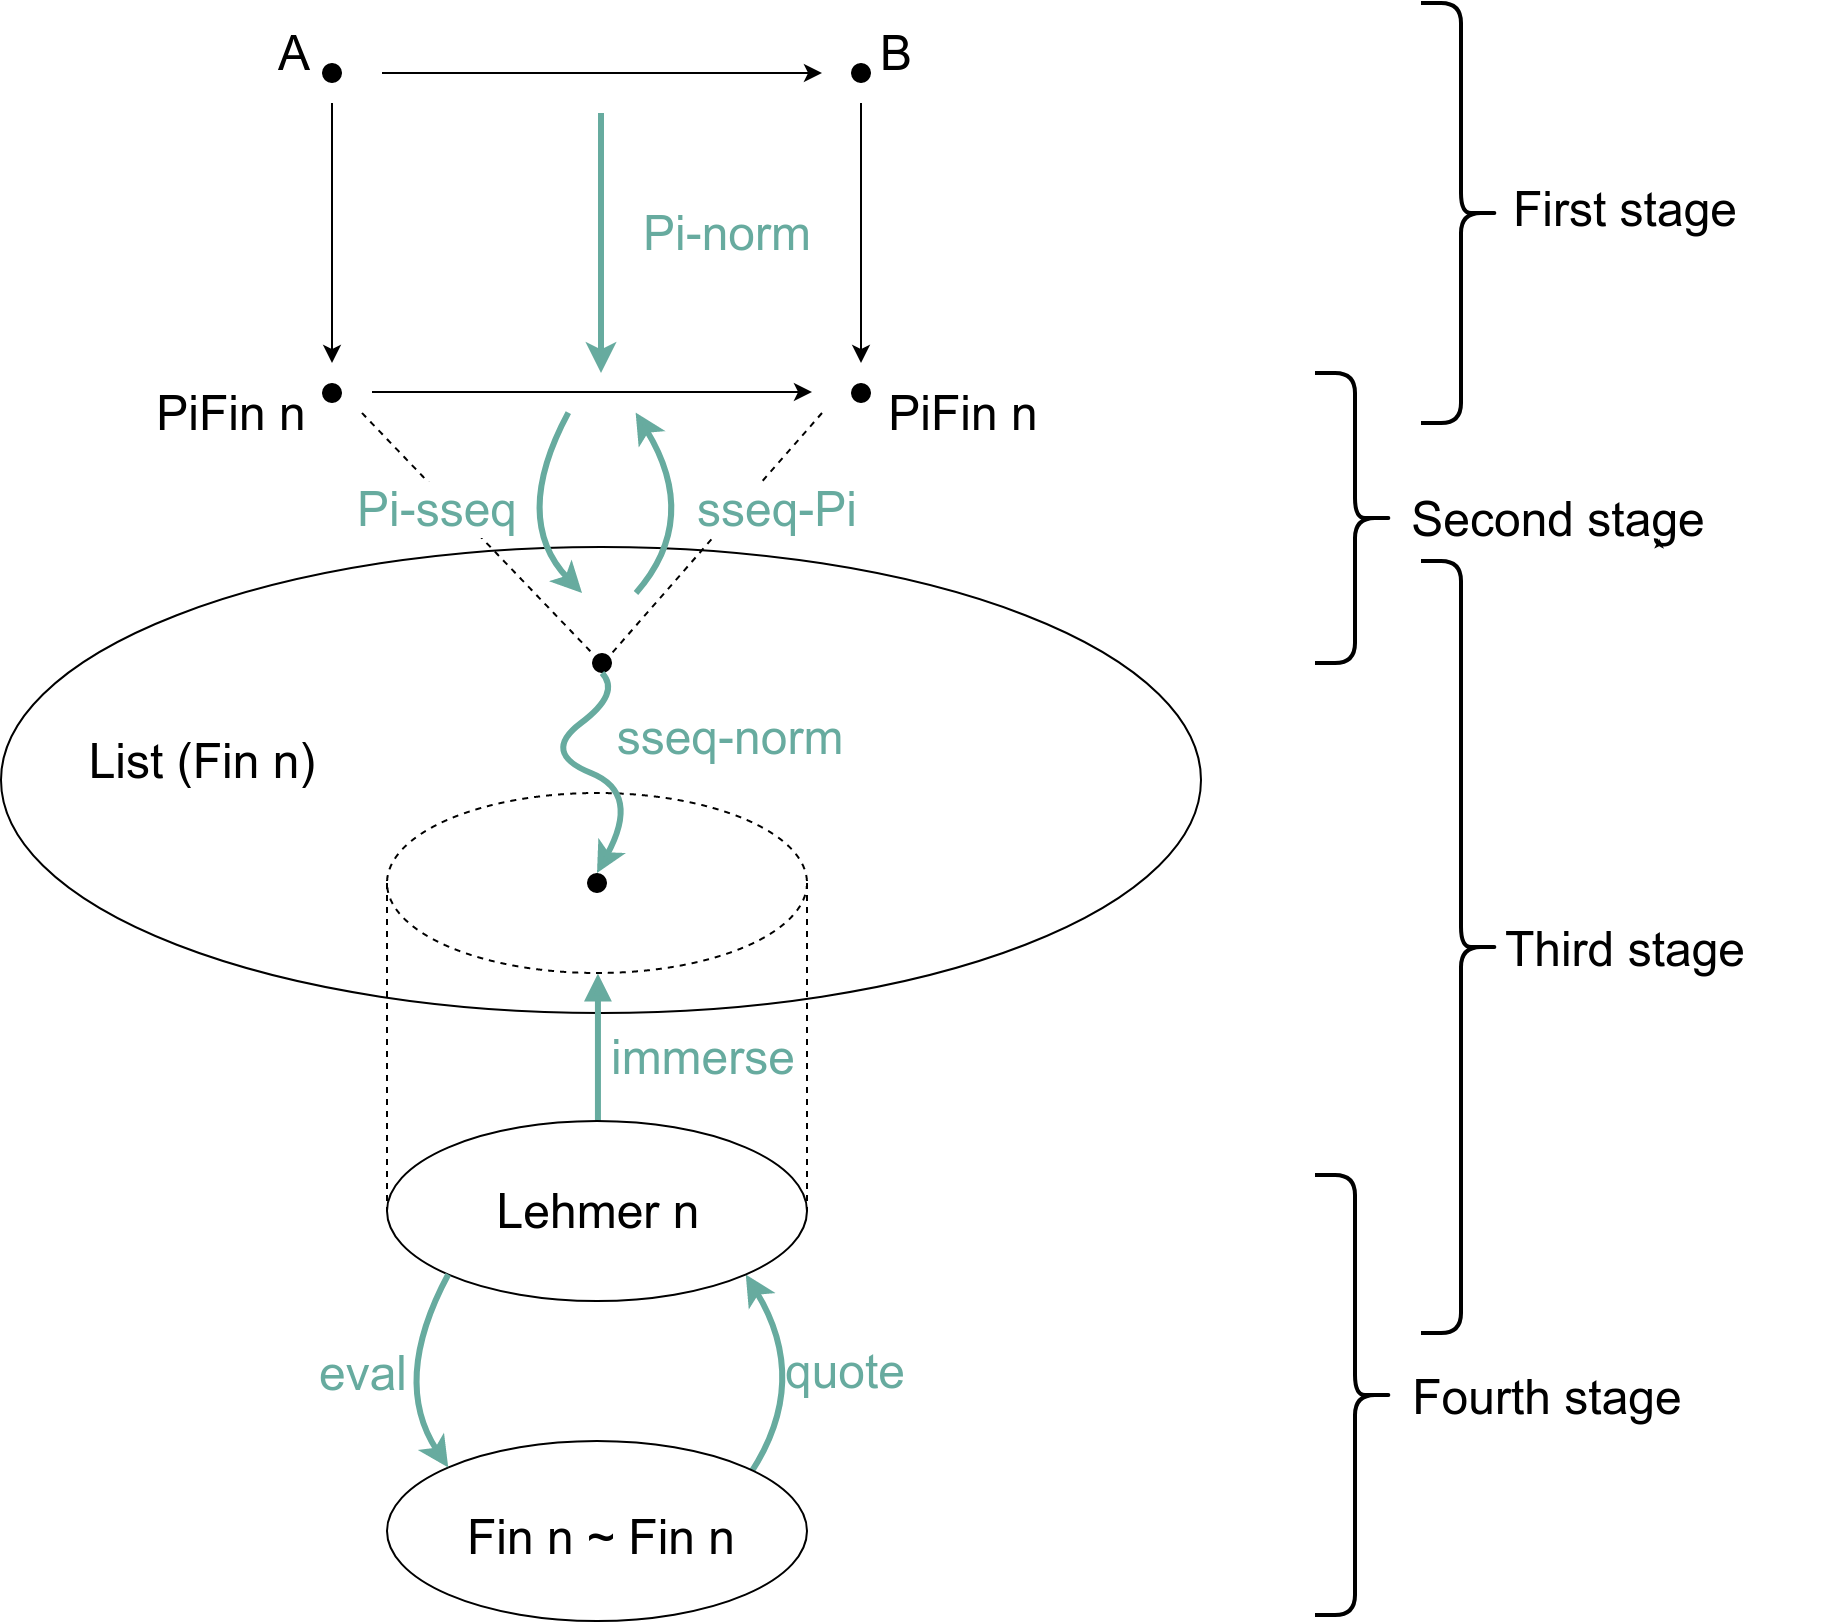
\includegraphics[scale=0.3]{outline.png}
% \end{center}

% \note{Redo this figure or delete ??}

%% \note{Spiel about reversible computing and logical reversibility ??}

%% \note{Spiel about using groupoids for denotational semantics ??}

%% \note{Could we include a short paragraph about entropy and bits and logical
%% reversibility ??}

%% \note{Novel interpretation of the univalence axiom, operational and
%% denotational semantics and adequacy.}

% * STLC(first) is the type theory for CCC
%   HoTT is type theory for weak infty groupoids(first)
%   Correspondence between TT and categories are fruitful:
%   answer hard questions about syntax without worrying about presentation
%   normalisation of lcal with strong sums: if you have specific syntax; no obvious induction on syntax
%   Lawvere thesis

% * Rig groupoids are interesting! WHY????
%   Add monoidal structure to weak groupoids. Easy. Lists
%   How symmetry is going to act on higher dimension
%   Higher-dim all symmetric; topology higher things abelian groups

%   * What is the corresponding type theory ?  We give it for the free symmetric
%   groupoid; for other groupoids build on it and add more

% The technical device to achieve this normalisation is as follows. First, we
% observe that 1-paths in $\UFin$ are permutations on finite sets with a fixed
% cardinality $n$, given by $\Aut[\Fin[n]]$, which produce the permutation group
% on $\Fin[n]$, or the symmetric group $\Sn$. By giving a presentation of $\Sn$
% using generators and relations, we build a rewriting system using the Coxeter
% relations~\cite{XXX} on the set of words $\List[\Fin[n]]$, and show that it is
% (locally) confluent and strongly normalising. We then establish that the
% symmetric group $\Sn$ is the set-quotient of $\List[\Fin[n]]$ by the Coxeter
% relations, and show that it produces a group presentation, as a quotient of
% the free group. Using this strongly normalising rewriting system, we establish
% that normal forms for words in $\Sn$ are Lehmer
% codes~, which are a convenient and
% compact representation of permutations. Finally, we show that there is an
% equivalence between Lehmer codes and permutations $\Aut[\Fin[n]]$ given by the
% Lehmer encode-decode algorithm.

%% ***
%%%%%%%%%%%%%%%%%%%%%%%%%%%%%%%%%%%%%%%%%%%%%%%%%%%%%%%%%%

%%% Local Variables:
%%% mode: latex
%%% TeX-master: "main"
%%% fill-column: 120
%%% End:
